\documentclass[a4paper]{report}
\usepackage[utf8]{inputenc}
\usepackage[portuguese]{babel}
\usepackage{hyperref}
\usepackage{a4wide}
\hypersetup{pdftitle={CC - TP01},
pdfauthor={João Teixeira, José Ferreira, Miguel Solino},
colorlinks=true,
urlcolor=blue,
linkcolor=black}
\usepackage{subcaption}
\usepackage[cache=false]{minted}
\usepackage{listings}
\usepackage{booktabs}
\usepackage{multirow}
\usepackage{appendix}
\usepackage{tikz}
\usepackage{authblk}
\usepackage{bashful}
\usepackage{verbatim}
\usepackage{amsmath}
\usepackage{tikz}
\usepackage{tikz,fullpage}
\usepackage{pgfgantt}
\usetikzlibrary{arrows,%
                petri,%
                topaths}%
\usepackage{tkz-berge}
\usetikzlibrary{positioning,automata,decorations.markings}
\AfterEndEnvironment{figure}{\noindent\ignorespaces}
\AfterEndEnvironment{table}{\noindent\ignorespaces}

\begin{document}

\title{Comunicação por Computadores\\ 
\large Fase 1 - Grupo 7}
\author{José Ferreira (A83683) \and João Teixeira (A85504) \and Miguel Solino (A86435)}
\date{\today}

\begin{center}
    \begin{minipage}{0.75\linewidth}
        \centering
        
\includegraphics[width=0.4\textwidth]{images/eng.jpeg}\par\vspace{1cm}
        \vspace{1.5cm}
        \href{https://www.uminho.pt/PT}
        {\color{black}{\scshape\LARGE Universidade do Minho}} \par
        \vspace{1cm}
        \href{https://www.di.uminho.pt/}
        {\color{black}{\scshape\Large Departamento de Informática}} \par
        \vspace{1.5cm}
        \maketitle
    \end{minipage}
\end{center}

\chapter{Questão 1}

\begin{table}[H]
\begin{tabular}{|l|l|l|l|l|}
\hline
\textit{\begin{tabular}[c]{@{}l@{}}Comando Usado\\ (Aplicação)\end{tabular}} &
  \begin{tabular}[c]{@{}l@{}}Protocolo de\\ Aplicação\end{tabular} &
  \begin{tabular}[c]{@{}l@{}}Protocolo de\\ transporte\end{tabular} &
  \begin{tabular}[c]{@{}l@{}}Porta de\\ atendimento\end{tabular} &
  \begin{tabular}[c]{@{}l@{}}Overhead de transporte\\ em bytes\end{tabular} \\ 
\hline
Ping         & -      & -   & -     & -  \\ \hline
Tracerout    & -      & UDP & 33446 & 8  \\ \hline  
telnet       & telnet & TCP & 23    & 20 \\ \hline 
ftp          & ftp    & TCP & 21    & 20 \\ \hline 
Tftp         & tftp   & UDP & 69    & 8  \\ \hline
browser/http & http   & TCP & 80    & 20 \\ \hline
ssh          & sshv2  & TCP & 22    & 20 \\ \hline
\end{tabular}
\end{table}

\begin{figure}[H]
    \centering 
    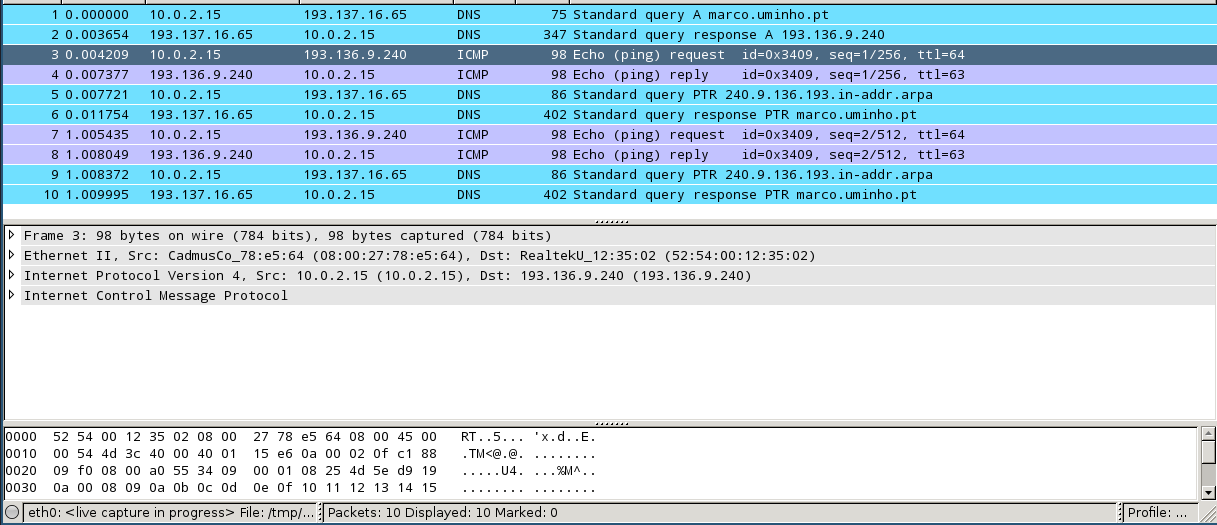
\includegraphics[width=\textwidth]{images/ping.png}  
    \caption{PING}
    \label{fig:ping}
\end{figure}

\begin{figure}[H]
    \centering 
    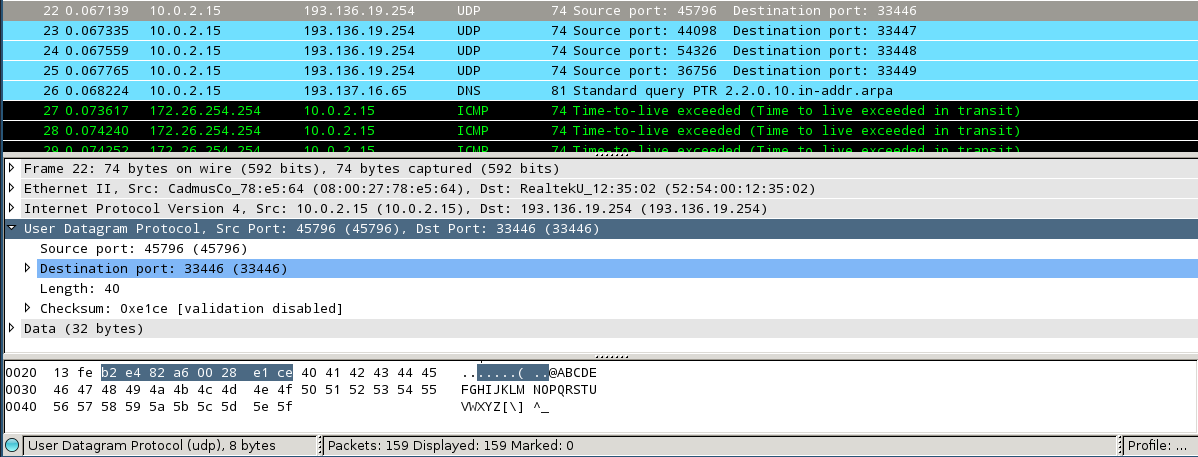
\includegraphics[width=\textwidth]{images/tracerout.png}  
    \caption{TRACEROUTE}
    \label{fig:tracerout}
\end{figure}

\begin{figure}[H]
    \centering 
    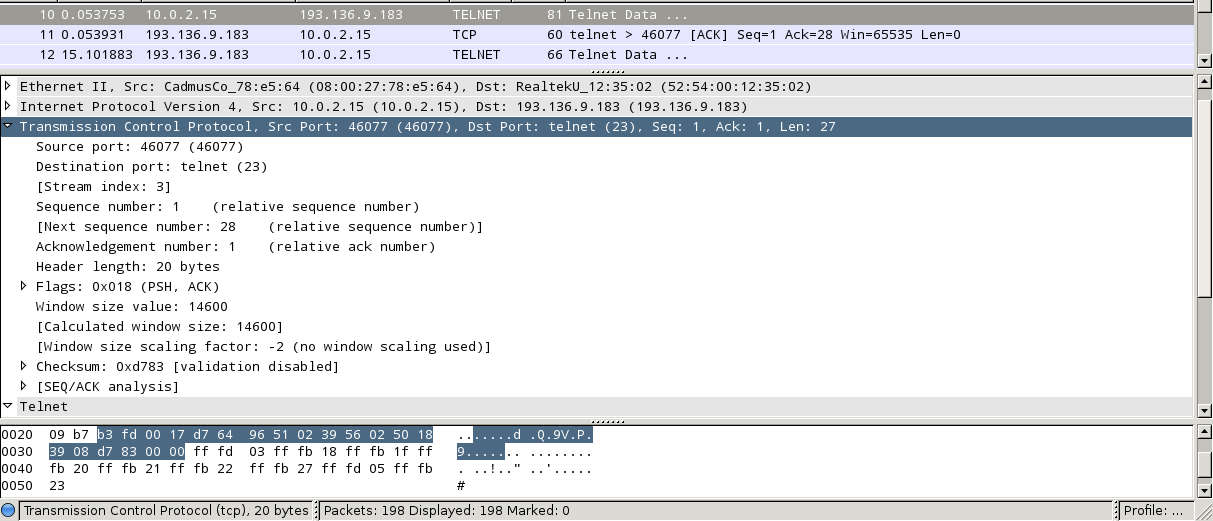
\includegraphics[width=\textwidth]{images/telnet.png}  
    \caption{TELNET}
    \label{fig:telnet}
\end{figure}

\begin{figure}[H]
    \centering 
    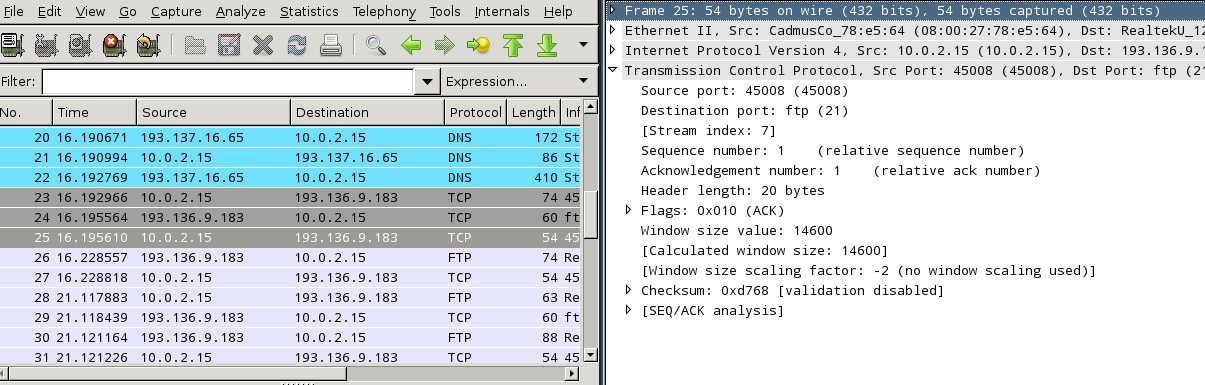
\includegraphics[width=\textwidth]{images/ftp.png}  
    \caption{FTP}
    \label{fig:ftp}
\end{figure}

\begin{figure}[H]
    \centering 
    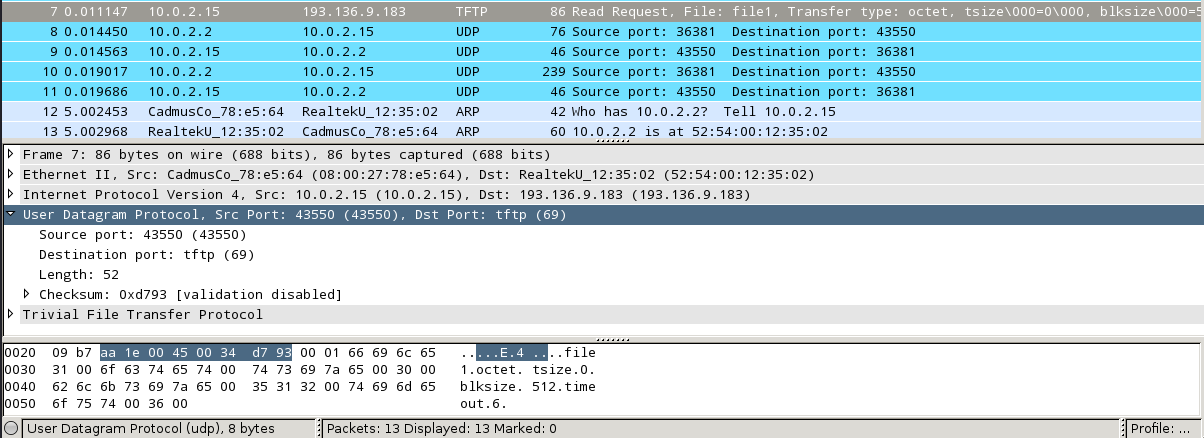
\includegraphics[width=\textwidth]{images/tftp.png}  
    \caption{TFTP}
    \label{fig:tftp}
\end{figure}

\begin{figure}[H]
    \centering 
    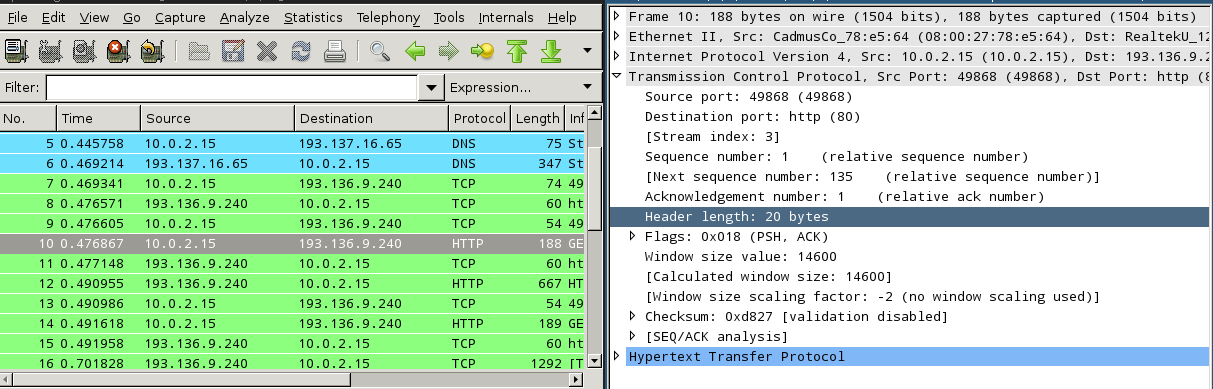
\includegraphics[width=\textwidth]{images/http_browser.png}  
    \caption{HTTP/browser}
    \label{fig:http_browser}
\end{figure}

\begin{figure}[H]
    \centering 
    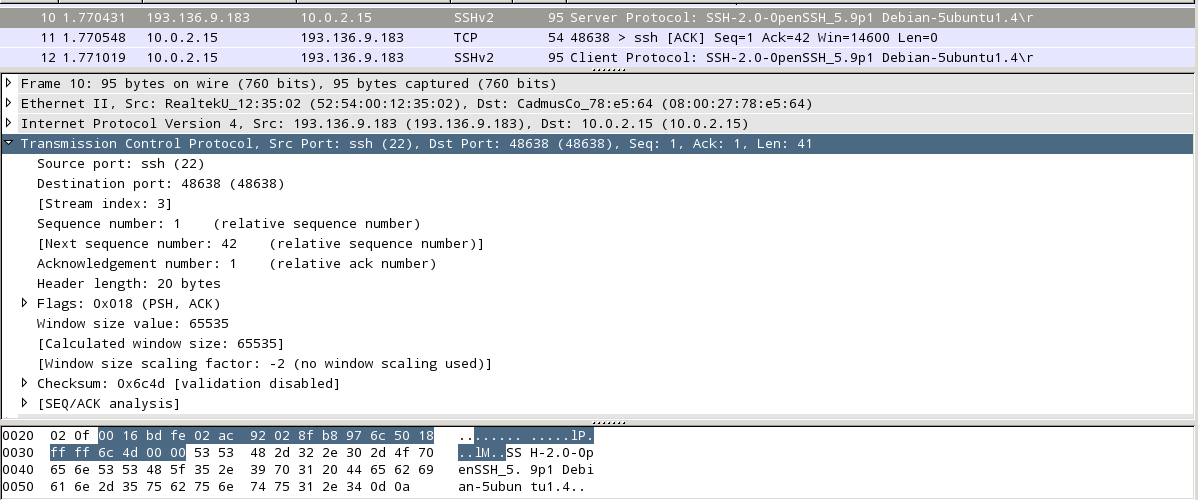
\includegraphics[width=\textwidth]{images/ssh.png}  
    \caption{SSH}
    \label{fig:ssh}
\end{figure}

\begin{figure}[H]
    \centering 
    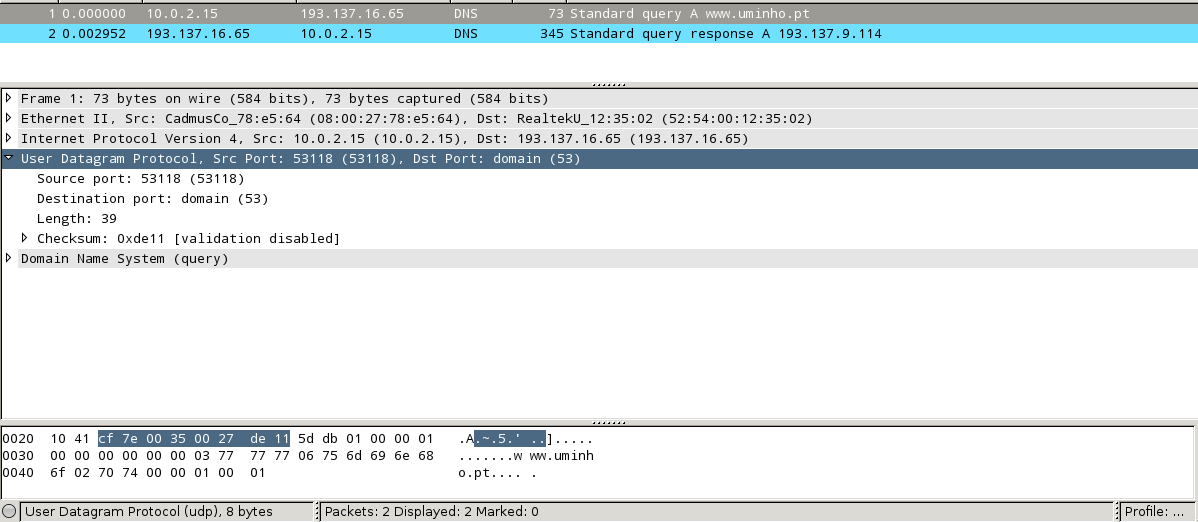
\includegraphics[width=\textwidth]{images/nslookup.png}  
    \caption{nslookup}
    \label{fig:NSLOOKUP}
\end{figure}

\chapter{Questão 2}
\textbf{Uma representação num diagrama temporal das transferências da file1 por
FTP e TFTP respetivamente. Se for caso disso, identifique as fases de
estabelecimento de conexão, transferência de dados e fim de conexão. Identifica
também claramente os tipos de segmentos trocados e os números de sequência
usados quer nos dados como nas confirmações.}

\begin{figure}[H]
    \centering 
    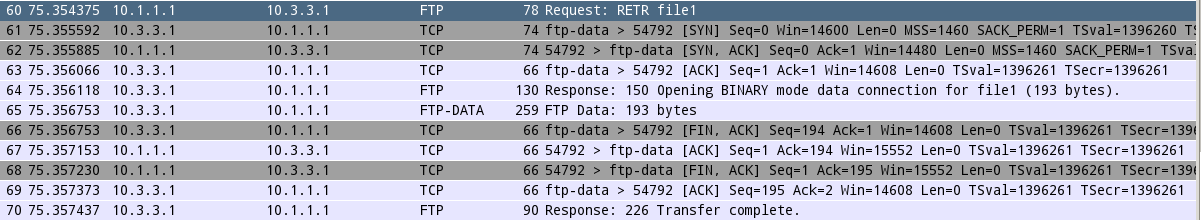
\includegraphics[width=\textwidth]{images/2ftp.png}  
    \caption{FTP}
    \label{fig:2ftp}
\end{figure}

\begin{figure}[H]
    \centering 
    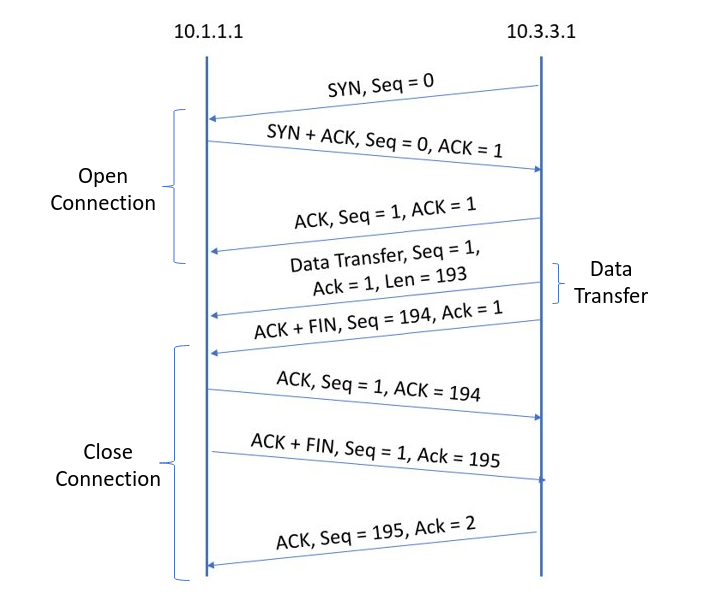
\includegraphics[width=0.6\textwidth]{images/diagrama.png}  
    \caption{FTP- Diagrama Temporal}
    \label{fig:diagrama}
\end{figure}

\begin{figure}[H]
    \centering 
    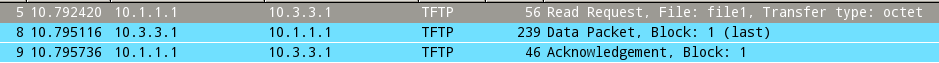
\includegraphics[width=\textwidth]{images/2tftp.png}  
    \caption{TFTP}
    \label{fig:2tft:}
\end{figure}

\begin{figure}[H]
    \centering 
    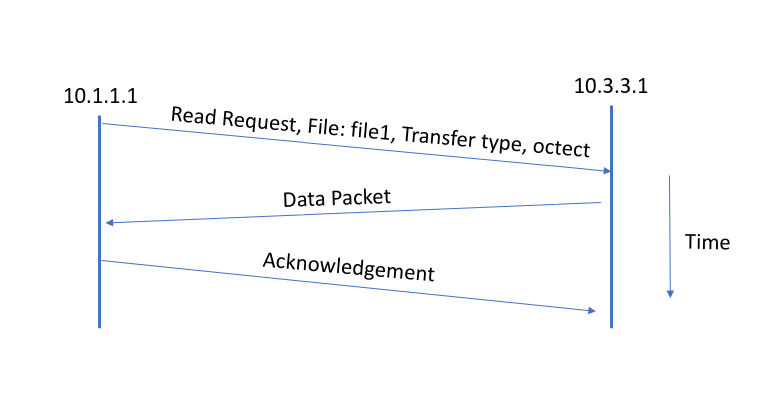
\includegraphics[width=0.6\textwidth]{images/diagrama2.png}  
    \caption{TFTP - Diagrama Temporal}
    \label{fig:diagrama2}
\end{figure}

\chapter{Questão 3}
\textbf{Com base nas experiências realizadas, distinga e compare sucintamente as
quatro aplicações de transferência de ficheiros que usou nos seguintes pontos
(i) uso da camada de transporte; (ii) eficiência na transferência; (iii)
complexidade; (iv) segurança;}

\section{SFTP}
\subsection{Uso da camada de transporte}
Protocolo TCP.

\subsection{Eficiência na transferência}
Devido à sua fiabilidade não é muito eficiente.

\subsection{Complexidade}
Disponibiliza várias funcionalidades. logo torna-se muito complexo.

\subsection{Segurança}
Recorre à autenticação e à encriptação dos dados, ou seja pode se dizer que é
seguro.

\section{FTP}
\subsection{Uso da camada de transporte}
Protocolo TCP.

\subsection{Eficiência na transferência}
Tem um maior overhead e isso deve-se a ser fiável.

\subsection{Complexidade}
Sendo que garante a segurança de transferência de dados, torna-se complexo.

\subsection{Segurança}
É pouco seguro, contudo utiliza autenticação.

\section{TFTP}
\subsection{Uso da camada de transporte}
Protocolo UDP.

\subsection{Eficiência na transferência}
Possui um overhead menor não se responsabilizando pela entrega dos dados.

\subsection{Complexidade}
Sendo que utiliza um protocolo UDP, as funcionalidades existentes não são
várias, logo não é muito complexo.

\subsection{Segurança}
Não utiliza qualquer mecanismo de autenticação ou encriptação, sendo assim pouco
seguro.

\section{HTTP}
\subsection{Uso da camada de transporte}
Protocolo TCP.

\subsection{Eficiência na transferência}
Possui uma grande eficiência.

\subsection{Complexidade}
Mesmo utilizando um protocolo TCP, trata-se de uma aplicação pouco complexa.

\subsection{Segurança}
Sendo que só utiliza autenticação, não é muito seguro.

\chapter{Questão 4}
\textbf{As características das ligações de rede têm uma enorme influência nos
níveis de Transporte e de Aplicação. Discuta, relacionando a resposta com as
experiências realizadas, as influências das situações de perda ou duplicação de
pacotes IP no desempenho global de Aplicações fiáveis (se possível, relacionando
com alguns dos mecanismos de transporte envolvidos).}

\begin{figure}[H]
    \centering 
    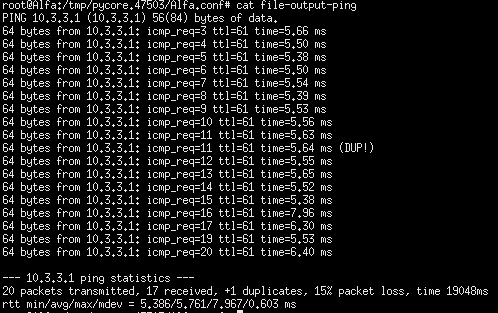
\includegraphics[width=0.7\textwidth]{images/4.png}  
    \caption{Ping}
    \label{fig:4}
\end{figure}
Observando a figura \ref{fig:4}, podemos ver que existiu 15\% de perda de pacotes e 1 foi duplicado. Maior parte das vezes isto
deve-se a existirem problemas ao nível da ligação de rede. Quando se trata de protocolos de transporte existem dois principais
que tratam deste problema de formas diferentes, sendo eles TCP e UDP. O primeiro é o mais complexo devido a utilizar mecanismos
de deteção e recuperação, garantindo que todos os pacotes são enviados na ordem correta e sem erros. Contudo, esta complexidade
também tem os seus defeitos. Como são trocados imensos pacotes por ambas as partes, quando nos encontramos numa rede de menor 
qualidade são corrompidos e perdidos. Com isso, são enviadas mensagens de erro e reenviados os pacotes originando numa maior
sobrecarga. Já a segunda é um protocolo muito menos complexo o que permite a própria a aplicação garantir que os dados são 
corretamente recebidos. No entanto, sendo pouco complexo não existe muito controlo caso os pacotes sejam perdidos, necessitando
que os protocolos acima do UDP identifiquem e corrijam o problema.

\chapter{Conclusão}
Na realização deste trabalho concluimos que maior parte dos conteúdos lecionados
nas aulas teóricas foram colocados em prática.\\
Na primeira parte foram vistos e aplicados vários protocolos de transporte e
aplicacionais.\\
Já na segunda, os conceitos TCP e UDP receberam uma maior atenção garantindo que
a nossa perceção dos mesmos ficasse clara.\\
As principais ferramentas utilizadas para que isto fosse possível foram o Core e
o Wireshark, sendo que maior parte do tempo utilizado para este TP foi na
análise de tráfego colocando em uso os vários protocolos de Aplicação e
Transporte.
\end{document}
